\documentclass[../main.tex]{subfiles}
\graphicspath{{\subfix{../IMAGES/}}}

\begin{document}
\localtableofcontents

\subsection{Introduction}

Water resources management is a primary engineering task to build dams, lay pipelines, install pumps and operate systems (1950 policy). Today : it must pursue sustainable development with measures that manage water for human system but at the same time protect the nature.\\

\begin{figure}[hbt!]
    \centering
    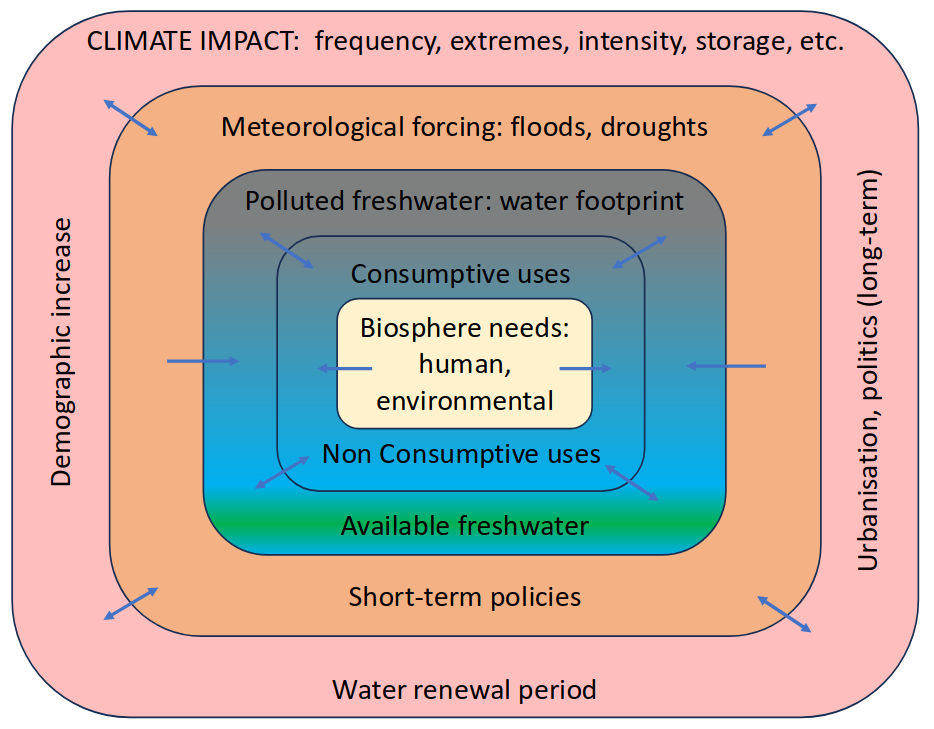
\includegraphics[width=0.5\linewidth]{IMAGES/Hydraulic/Screenshot from 2025-02-17 14-22-06.png}
\end{figure}

\begin{theorem}
    Scarcity : imbalance of supply/demand under given institutional/economic/social boundary conditions (relative concept).\\
    Shortage : low level of supply relative to minimum level for basic needs (absolute concept).\\
    Stress : symptom of water scarcity/shortage (conflict between user, competition for water).\\
\end{theorem}

Factors affecting water scarcity : \begin{itemize}
    \item Hydrologic/climate origin
    \item Anthropic origin : water quality maintenance due to water uses, high living standards increase WS, technology level of a County.
\end{itemize}

Water security is a term that refers to a society's capacity to have enough water of sufficient quality for survival and to carry out different development actions.\\

The use of water colors it : blue water (river, lakes, glaciers, ...), green water (forests, soil moisture, cultures, ...), gray water (domestic use, industrial, ...).\\
\warning The output from any process is always gray water. \\

Virtual water reflects the amount of water physically contained in the product is negligible compared to the amount that went into its production. It allows precise and practical applications since the amounts of water that goes into production processes can be quantified.\\

\begin{theorem}
    States that are crossed or that share entirely or partially a water course are called \textbf{Riparian States}.\\
    Riparian states have incommensurable responsibilities vs downstream countries. 
\end{theorem}

Strengthening global water initiatives (GWIs) are proficient at their best and weak and corrupt and their worst. 



\end{document}